
\newpage
\subsection{A priori estimates}%
\label{sec:a_priori_estimates}


In this section, we will only briefly overview the important assumptions and definitions and then prove that the ghost penalty does affect the convergence rate specifically for the energy norm.
However, the $C^{0}$ discrete solution is to rough for the standard Lagrange interpolation operator. Hence, this motivates us to introduce a method to interpolate a non-smooth function, the so-called Cléments interpolation operator.

\subsubsection{Cléments interpolation}%
\label{ssub:clement_operator}

\begin{figure}
\begin{minipage}{.5\linewidth}
\centering
\subfloat[]{
    \label{fig:macroelements:a}
    \begin{tikzpicture}[scale=0.5]
        % Arbitrary triangle
        \coordinate (A1) at (0,0);
        \coordinate (B1) at (4,1);
        \coordinate (C1) at (1,3);
        \fill [red!30] (A1) -- (B1) -- (C1) -- cycle;
        \draw (A1) -- (B1) -- (C1) -- cycle;

        % Centroid
        \coordinate (ai) at (barycentric cs:A1=1,B1=1,C1=1);
        \fill (ai) circle (2pt);
        \node[anchor=north west] at (ai) {$a_i$};

        % Reference triangle
        \coordinate (A2) at ($(A1) + (6, 0)$);
        \coordinate (B2) at ($(A2) + (0, 3)$);
        \coordinate (C2) at ($(A2) + (3, 0)$);
        \fill [blue!30] (A2) -- (B2) -- (C2) -- cycle;
        \draw (A2) -- (B2) -- (C2) -- cycle;

        % Centroid of the reference triangle
        \coordinate (ahi) at (barycentric cs:A2=1,B2=1,C2=1);
        \fill (ahi) circle (2pt);
        \node[anchor=north west] at (ahi) {$\hat{a}_{j( i)} $};

        \draw[->, thick, >=stealth] ($(ahi)+(0.2,+0.2)$) to[bend right] node[midway, above] {$G_{A_i}$} ($(ai)+(0.2,+0.3)$);

    \end{tikzpicture}
}
\end{minipage}%
\begin{minipage}{.5\linewidth}
\centering
\subfloat[]{
    \label{fig:macroelements:b}
    \begin{tikzpicture}[scale=0.5]
    % Arbitrary square
    \coordinate (A1) at (0,0);
    \coordinate (B1) at (3,1);
    \coordinate (C1) at (4,4);
    \coordinate (D1) at (1,3);
    \draw (A1) -- (B1) -- (C1) -- (D1) -- cycle;
    \fill[red!30] (A1) -- (B1) -- (C1) -- (D1) -- cycle;

    % Draw edge from D1 to B1
    \draw (D1) -- (B1);

    % Pick a point on the edge and label it as a_i
    \coordinate (a_i) at ($(D1)!.6!(B1)$);
    \fill (a_i) circle (2pt);
    \node[anchor=north] at (a_i) {$a_i$};

    % Reference equilateral triangle
    \coordinate (A2) at ($(A1) + (6, 0)$);
    \coordinate (B2) at ($(A2) + (2, 3.464)$); % 3.464 = 2 * sqrt(3)
    \coordinate (C2) at ($(A2) + (4, 0)$);
    \fill[blue!30] (A2) -- (B2) -- (C2) -- cycle;
    \draw (A2) -- (B2) -- (C2) -- cycle;

    % Divide the equilateral triangle into two right triangles
    \coordinate (M) at ($(A2)!.5!(C2)$);
    \draw (B2) -- (M);

    % Pick a point on the shared edge and label it as ahat_i
    \coordinate (ahat_i) at ($(B2)!.7!(M)$);
    \fill (ahat_i) circle (2pt);
    \node[anchor=north west] at (ahat_i) {$\hat{a}_{j( i)} $};

    % Draw the mapping G_{A_i} from ahat_i to a_i
    \draw[->, thick, >=stealth] ($(ahat_i)+(0.2,0.2)$) to[bend right] node[midway, above] {$G_{A_i}$} ($(a_i)+(0.2,0.2)$);
\end{tikzpicture}
}
\end{minipage}\par\medskip
\centering
\subfloat[]{
    \label{fig:macroelements:c}
 \begin{tikzpicture}[scale=0.5]

    % Central vertex a_i
    \coordinate (ah_i) at (0, 0);

    % Reference hexagon
    \foreach \angle in {0, 60, ..., 300} {
        \coordinate (A) at (\angle:2.5);
        \coordinate (B) at (\angle + 60:2.5);
        \fill[blue!30] (ah_i) -- (A) -- (B) -- cycle;
        \draw (ah_i) -- (A) -- (B) -- cycle;
    }

    \fill (ah_i) circle (2pt);
    \node[anchor=east, yshift=0.25cm] at (ah_i) {$\hat{a}_{j( i) }$};

    \coordinate (A1) at (5, 0);
    \coordinate (B1) at (8, 0);
    \coordinate (C1) at (8, 3);
    \coordinate (D1) at (7, 4);
    \coordinate (E1) at (3.5, 4);
    \coordinate (F1) at (3, 2);
    \fill[red!30] (A1) -- (B1) -- (C1) -- (D1) -- (E1) -- (F1) -- cycle;
    \draw (A1) -- (B1) -- (C1) -- (D1) -- (E1) -- (F1) -- cycle;

    \coordinate (ai) at (barycentric cs:A1=1,B1=1,C1=1,D1=1,E1=1,F1=1);
    % Draw lines from vertices to a_i
    \draw (A1) -- (ai);
    \draw (B1) -- (ai);
    \draw (C1) -- (ai);
    \draw (D1) -- (ai);
    \draw (E1) -- (ai);
    \draw (F1) -- (ai);
    % Centroid
    \fill (ai) circle (2pt);
    \node[anchor=south, yshift=0.2cm] at (ai) {$a_i$};

    \draw[->, thick, >=stealth] ($(ah_i)+(0.2,- 0.2)$) to[bend right] node[midway, above, yshift=0.1cm] {$G_{A_i}$} ($(ai)+(-0.2,-0.2)$);

\end{tikzpicture}
}

\caption{Illustration of the different cases when mapping from the reference macroelement $\widehat{A}_{j( i) }$  to the domain $A_{i}$,  $G_{A_{i}}: \widehat{A}_{j( i) } \to A_{i}$. Here we have defined $\hat{a}_{j(i)} \in \widehat{A}_{j(i)}$ s.t. $G( \hat{a}_{j( i) })
= a_i$. }

\label{fig:macroelements}
\end{figure}


We want to compute the expected convergence rate of the energy norm \eqref{eq:bi_Ah_norm}. An important tool in the process is the Cléments interpolation operator, $C_{h}$.
It is used for interpolation on non smooth functions by applying an regularization on so-called macroelements. Let us denote the $\mathcal{P}_{c}^{k}( \Omega )  $ to be an $H^{1}$ conformal polynomial space. We denote $\left\{ a_{1}, \ldots, a_{N}
\right\} $ to be the Lagrange nodes. Associated with each node $a_{i}$ we denote the macroelement $A_{i}$ to consist of all simplices containing $a_{i}$. Let $n_{cf}$ be the number of configurations for the macroelement, then we define the index $j:
\left\{ 1,\ldots,N \right\} \to \left\{ 1, \ldots, n_{cf} \right\}  $ s.t. $j( i) $ is the index associated with the reference configuration $\widehat{A}_{j(i) }$ for corresponding macroelement $A_{i}$ for an illustration, see
Figure \ref{fig:macroelements}.

Let us define a $C^{0}$-diffeomorphism $G_{A_{i}}:
\widehat{A}_{j( i) } \to A_{i}$ s.t. for all $\widehat{T} \in \widehat{A}_{j( i) } $ is the restriction $G_{A_{i}  \mid \widehat{T}}$ affine. The Cléments interpolation operator $C_{h}$ is defined as a $L^2$-projection onto the macroelements. That is, given
a reference macroelement $\widehat{A}_{j( i) }$ and a function $\hat{v} \in L^{1}( \widehat{A}_{j( i) })  $, then $\widehat{C}_{j( i) } \hat{v}$  is the unique polynomial in $\mathcal{P}^{k} ( \widehat{A}_{j( i) })  $ s.t. \[
\int_{  \widehat{A}_{j( i) }}^{} ( \widehat{C}_{j( i) } \hat{v} - \hat{v}) p \ dx  = 0 \quad  \forall p \in \mathcal{P}^{k} ( \widehat{A}_{j( i) })
\]
Finally, we define the Cléments interpolator $C_{h} : L^{1}( \Omega )  \to \mathcal{P} ^{k}_{c}(\Omega  ) $ s.t.
\[
C_{h} v = \sum_{i=1}^{N} \widehat{C}_{j( i) } ( v (G_{A_{i}}) (G^{-1}_{A_{i}}(a_{i})) )\phi _{i},
\]
where $\phi _{i}$ is the corresponding polynomial basis at node $a_{i}$.

Recall the integral norm notation,
\[
\| u \|_{ m,p,T }^{  } = \left( \sum_{ \left\lvert \alpha  \right\rvert \le m}^{} \int_{T}^{}  \left\lvert  \partial ^{\alpha } u \right\rvert^{p} dx   \right)^{\frac{1}{2}}
\]
where we use that $\| u \|_{ T  }^{  } = \| u \|_{ m,0,T  }^{  } $ and similarly $\| u \|_{ 2,T  }^{  } = \| u \|_{ m,2,T  }^{  }  $.

We denote a patch, $\omega \left( T \right) $, as the set of elements in $\mathcal{T} _{h}$  sharing at least one vertex with $T \in \mathcal{T} _{h}$ . And similarly we denote a another patch, $\omega \left( F \right) $, as the set of all elements in $\mathcal{T}_{h} $
sharing at least one vertex with $F \in  \mathcal{F} _{h}$. For an example of patches a triangular mesh in 2D, see Figure \ref{fig:example_path}.


\begin{figure}[ht]
    \centering

  \centering
    \subfloat{{
    \begin{minipage}[b]{0.45\textwidth}
        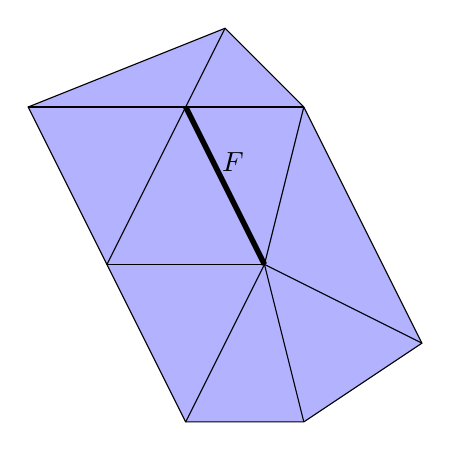
\begin{tikzpicture}
            % Define the coordinates
            \coordinate (A) at (0,0);
            \coordinate (B) at (2,0);
            \coordinate (C) at (1,2);
            \coordinate (D) at (2.5,2);
            \coordinate (F) at (1.5,3);
            \coordinate (E) at (-1,2);
            \coordinate (G) at (1,-2);
            \coordinate (H) at (2.5,-2);
            \coordinate (I) at (4,-1);

            \fill[blue!30] (A) -- (G)-- (H) -- (I)  -- (D) -- (F)-- (E)   -- cycle;

            % Draw the triangle
            \draw (A) -- (G)-- (H) -- (I)  -- (D) -- (F)-- (E)   -- cycle;
            \draw (A) -- (C);
            \draw (A) -- (B);
            \draw (G) -- (B);
            \draw (I) -- (B);
            \draw (F) -- (C);
            \draw (H) -- (B);
            \draw (D) -- (C);
            \draw (D) -- (B);
            \draw (E) -- (C);
            \draw[line width=2pt] (B) -- (C);
            \node at (1.6,1.3) {$F$};

        \end{tikzpicture}
    \end{minipage}\hfill

}}%
    \qquad
    \subfloat{{

    \begin{minipage}[b]{0.45\textwidth}
        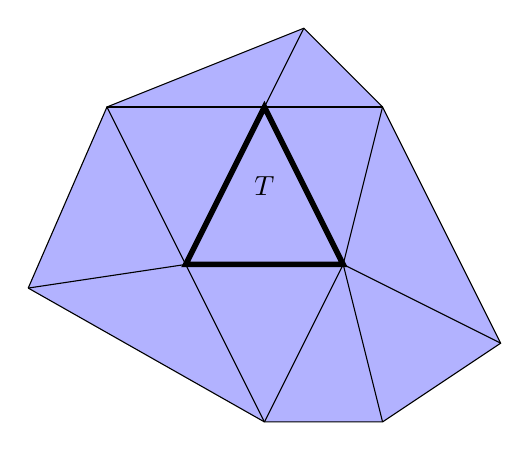
\begin{tikzpicture}
                    % Define the coordinates
        \coordinate (A) at (0,0);
        \coordinate (B) at (2,0);
        \coordinate (C) at (1,2);
        \coordinate (D) at (2.5,2);
        \coordinate (F) at (1.5,3);
        \coordinate (E) at (-1,2);
        \coordinate (G) at (1,-2);
        \coordinate (H) at (2.5,-2);
        \coordinate (I) at (4,-1);
        \coordinate (K) at (-2,-0.3);

        \fill[blue!30] (K) -- (G)-- (H) -- (I)  -- (D) -- (F)-- (E)   -- cycle;
        % \fill[red!30] (B) -- (C) -- (A);

        % Draw the triangle
        \draw (A) -- (G)-- (H) -- (I)  -- (D) -- (F)-- (E)   -- cycle;
        \draw (A) -- (C);
        \draw (A) -- (B);
        \draw (G) -- (B);
        \draw (I) -- (B);
        \draw (F) -- (C);
        \draw (H) -- (B);
        \draw (D) -- (C);
        \draw (D) -- (B);
        \draw (E) -- (C);
        \draw (K) -- (A);
        \draw (K) -- (G);
        \draw (K) -- (E);
        \draw[line width=2pt] (B) -- (C) -- (A) -- cycle;
        \node at (1.0,1.0) {$T$};

        \end{tikzpicture}
    \end{minipage}

    }}%
\caption{Illustration of the patch $\omega ( F) $ on the left-hand side and $\omega(T)$ on the right-hand side.}
    \label{fig:example_path}%
\end{figure}

Finally, we have the following lemma

\begin{lemma}
    \label{lemma:clements}

We define the Clement interpolation as the projection
$C_{h}: H^{m} \left( \Omega  \right) \mapsto V_{h}$, where $V_{h}$ has the order $k$. Then does the following stability estimate hold,
\[
 \| C_{h} v \|_{H^{m}\left( \Omega  \right)   }^{  } \lesssim \| v \|_{ H^{m}\left( \Omega  \right)  }^{  } \quad \forall v \in H^{m}\left( \Omega  \right),
\]
and if the following conditions for an parameter $l$ is satisfied, it exists error estimates s.t.,
\[
    \begin{split}
      m\le l \le k+1  \implies \| v - C_{h} v \|_{ m,p,T   }^{  }  &  \lesssim h^{l-m}_{T} \| v \|_{l,p,\omega \left( T \right)  }^{  } \quad  \forall T \in \mathcal{T} _{h}, \forall v \in H^{l}( \omega \left( T \right)
      ), \\
      m +\frac{1}{2}\le l \le k+1  \implies \| v - C_{h} v \|_{ m,p,F }^{  } & \lesssim h^{l-m- \frac{1}{2}}_{T} \| v \|_{l,p,\omega \left( F \right)  }^{  } \quad  \forall \partial T \in \mathcal{T} _{h}, \forall v \in H^{l}( \omega \left( F
      \right)).
    \end{split}
\]

\end{lemma}


\begin{corollary}
    \label{cor:celement_apriori}
    Let $0 \le l \le k+1$ and let $0\le m \le \min_{} ( 1,l )$.
    Given Lemma \ref{lemma:clements}  then there exists an $C > 0$ s.t.
    \[
    \inf_{v_{h} \in \mathcal{P} ^{k}_{c}( \Omega ) } \| v - v_{h} \|_{  m,p,\Omega }^{  } \le C h^{l-m}  \| v \|_{ l,p,\Omega  }^{  }    \forall v \in W_{l,p}( \Omega ).
    \]
\end{corollary}


This result is very useful since it is now sufficient to show that a priori estimates holds given to prove convergence rate.

For further detailed information about the Cléments interpolation, please investigate \cite[Chapter 1.6]{ern04}.
We will use these estimates to compute convergence rate given that Ceas' Lemma holds.


\subsubsection{Energy a priori estimates.  }%
\label{ssub:extension}
Recall that for $v \in H^{1}( \mathcal{T } _{h}) $ these inequalities holds $\forall T \in \mathcal{T} _{h}$ s.t. \[
\begin{split}
    \| v \|_{ \partial T }^{  } &\lesssim h^{-\frac{1}{2}}_{T}\|  v \|_{ T }^{  }+ h^{\frac{1}{2}} \| \nabla v \|_{T  }^{   }  , \\
    \| v \|_{ \Gamma \cap T }^{  } &\lesssim  h^{-\frac{1}{2}} \| v \|_{T  }^{  }   + h^{\frac{1}{2}}_{T} \| \nabla v \|_{ T }^{  }.
\end{split}
\]
For proof, see \cite[Lemma 4.2]{hansbo2003finite}.

A key idea is to distinguish between the physical space $\Omega $ and the polyhedra consisting of the active mesh $\Omega ^{e}_{h} = \mathcal{T}_{h}$. Thus, to do an
a priori estimate we find it necessary to define an bounded extension operator satisfying, \[
( \cdot ) ^{e}: W^{m,q}( \Omega )  \to W^{m,q} ( \Omega ^{e}), \quad \| v^{e} \|_{ m,q,\Omega ^{e}  }^{  } \lesssim \| v \|_{ m,q, \Omega  }^{  }.
\]
where $0< m \le \infty$ and $1 \le q \le \infty$.
\todo[inline]{ The physical space $\Omega $ is a subset of $\Omega ^{e}$, so I do not understand why $\| v^{e} \|_{ m,q,\Omega ^{e}  }^{  } \lesssim \| v \|_{ m,q, \Omega  }^{  } $ should hold.  I may also make a figure to illustrate $\Omega ^{e}$. }

Now assume that $\Omega _{h}^{e} \subset  \Omega^{e} $. We define an unfitted Cléments interpolator $C_{h}^{e}: H^{r}( \Omega ^{e}_{h}) \to V_{h}$
s.t.  $C ^{e} _{h} v := C _{h} v^{e} $.
We can immediately observe that the interpolation satisfies the global error estimates, that is,
\begin{align}
    \label{eq:bi_projection_estimates_1}
    \| v - C _{h}^{e} v \|_{  r, \mathcal{T} _{h} }^{  } & \lesssim h^{s-r}\sum_{T \in \mathcal{T}_h} \| v \|_{ s, \omega(T) }^{  }, \quad 0\le r\le s \\
    \label{eq:bi_projection_estimates_2}
\| v - C ^{e}_{h}v \|_{ r,\mathcal{F} _{h} }^{  } & \lesssim h^{s-r-\frac{1}{2}}\sum_{T \in \mathcal{T}_h} \| v \|_{ s, \omega(F)  }^{  }, \quad 0  \le  r \le   s- \frac{1}{2} \\
    \label{eq:bi_projection_estimates_3}
\| v - C ^{e}_{h}v \|_{ r, \Gamma }^{  } & \lesssim h^{s-r-\frac{1}{2}} \sum_{T \in \mathcal{T}_h}  \| v \|_{ s,  \omega(T)  }^{  }, \quad 0  \le  r \le   s- \frac{1}{2}
\end{align}

Naturally can we see this is the tools we need to construct an estimate for the energy norm.

\begin{lemma}
    \label{lemma:astar_estimate}
    Let $u \in H^{s}( \Omega ) $ for $s\ge 3$ be a exact solution. Then we have  \[
    \|  u - C_{h}u \|_{ a_{h},*  }^{  } \lesssim h^{s(s-2)} \| u \|_{ H^{s}( \Omega )  }^{  }
    \]

\end{lemma}
\begin{proof}
    By definition is
    \[
        \begin{split}
            \| u - C_{h}^{e}u \|_{ a_{h}, * }^{  2}  =& \ \| |\alpha |^{\frac{1}{2}} ( u - C_{h}^{e}u) \|_{ \mathcal{T} _{h} \cap \Omega  }^{ 2}  + \| D^2 ( u - C_{h}^{e}u ) \|_{\mathcal{T} _{h} \cap \Omega   }^{ 2 } \\  &  + \gamma \| h^{-\frac{1}{2}} \jump{ \partial _{n} (u -
        C_{h}^{e} u) }   \|_{ \mathcal{F}_{h}^{}\cap \Omega    }^{ 2
        } + \gamma \| h^{-\frac{1}{2}}  \partial _{n} (u - C_{h}^{e}u)    \|_{ \Gamma   }^{ 2 } \\
          & + \| h^{\frac{1}{2}} \mean{ \partial _{nn} (u - C_{h}^{e}u) }   \|_{\mathcal{F} _{h}^{} \cap \Omega   }^{  2} +  \| h^{\frac{1}{2}} \partial _{nn}(u - C_{h}^{e}u)     \|_{ \Gamma }^{  2}.
        \end{split}
    \]

    The strategy is to bound each term individually by applying the estimates \eqref{eq:bi_projection_estimates_1}, \eqref{eq:bi_projection_estimates_2} and \eqref{eq:bi_projection_estimates_2}.
    \begin{enumerate}[label=\arabic*)]
        \item     Starting with the first term we get
    \[
            \| |\alpha |^{\frac{1}{2}} ( u - C_{h}^{e}u) \|_{ \mathcal{T} _{h} \cap \Omega  }^{ 2}  \le  \| \alpha  \|_{L^\infty ( \Omega )    }^{2  }   \|  ( u - C_{h}^{e}u) \|_{0,\mathcal{T} _{h}  }^{ 2} \lesssim  h^{2s} \sum_{T \in \mathcal{T}
            _{h}}^{}   \| v \|_{s,w( T)  }^{  2}
    \]
    Here we simply used \eqref{eq:bi_projection_estimates_1}.
\item
    Similarly can we use  for the second term, \[
    \| D^2 ( u - C_{h}^{e}u ) \|_{\mathcal{T} _{h} \cap \Omega   }^{ 2 } \lesssim  \|  u - C_{h}^{e}u  \|_{2,\mathcal{T} _{h}   }^{ 2 } \lesssim \sum_{T \in \mathcal{T} _{h}}^{} h^{2(s-2)} \| u \|_{ s, \omega ( T)  }^{ 2 }.
    \]
    Again, this is via the estimate \eqref{eq:bi_projection_estimates_1}.
\item
        Recall $\| \jump{ u }   \|_{ \mathcal{F} _{h} }^{  } \le \| v^{+}   \|_{ \mathcal{F} _{h} }^{  } +   \| v^{-}   \|_{ \mathcal{F} _{h} }^{  } \lesssim  \| u \|_{ \partial\mathcal{T }_{h}  }^{2  }  $ and the inverse estimate $\| \partial _{n} u \|_{ F  }^{} \lesssim h^{-\frac{1}{2}} \| \nabla u \|_{ T }^{  }  $.
     Hence, by \eqref{eq:bi_projection_estimates_2}  \[
        \begin{split}
            \gamma \| h^{-\frac{1}{2}} \jump{ \partial _{n} ( u - C_{h}^{e}u ) }   \|_{ \mathcal{F}_{h} \cap \Omega   }^{  2}   &\lesssim \| h^{-\frac{1}{2}}  \partial _{n} ( u - C_{h}^{e}u )    \|_{  \partial \mathcal{T} _{h} }^{2  }
       \lesssim h^{-2} \|   \nabla  ( u - C_{h}^{e}u )    \|_{  \mathcal{T} _{h} }^{2  }     \\
                                                                                                                 &\lesssim h^{-2} \|      u - C_{h}^{e}u     \|_{1,  \mathcal{T}_{h} }^{2  }
                                                                                                                 \lesssim \sum_{T \in \mathcal{T} _{h}}^{} h^{2(s-1)} \| u \|_{ s,T  }^{ 2}
        \end{split}
    \]
    \todo[inline]{
        Not sure if \eqref{eq:bi_projection_estimates_2} holds here!
        \[
     \| \partial _{n}(u - C_{h}^{e}u)     \|_{1, \partial \mathcal{T}_{h} }^{2  }
                                                                                                                 \lesssim \sum_{T \in \mathcal{T}_{h} }^{}
                                                                                                                 h^{ 2(l - m - \frac{1}{2})  } \| u      \|_{ s, \omega (  F)  }^{  2}
    \]  }
\item
    And for the boundary term we simply apply \eqref{eq:bi_projection_estimates_3}, \[
        \begin{split}
            \gamma \| h^{-\frac{1}{2}}  \partial _{n} ( u - C_{h}^{e}u ) \|_{ \Gamma    }^{  2} \lesssim h^{-2} \|   \nabla  ( u - C_{h}^{e}u )    \|_{ \Gamma  }^{2  } \lesssim  h^{-2} \|    u - C_{h}^{e}u     \|_{1, \Gamma  }^{2  }\lesssim h^{2(s- r-
            \frac{1}{2}) -2}
              \sum_{T \in \mathcal{T} _{h}}^{}  \| u \|_{s,T  }^{  2}
        \end{split}
    \]
    \todo[inline]{ Does it makes sense to integrate $\| \nabla u \|_{ \Gamma  }^{  } $, i.e. no normal vectors? I guess not. Hence, \eqref{eq:bi_projection_estimates_3} is kinda strange.}
\item

            We also know that $\| \mean{ u }   \|_{ \mathcal{F} _{h} }^{  } \le \| u^{+} \|_{ \mathcal{F} _{h}  }^{  } + \| u^{-} \|_{ \mathcal{F} _{h}  }^{  }   \lesssim  \| u \|_{ \partial\mathcal{T }_{h}  }^{2  }  $ and the $\| \partial _{nn} u \|_{ F  }^{} \lesssim h^{-\frac{1}{2}} \| D^2 u \|_{ T }^{  }  $. It is clear
            by using \eqref{eq:bi_projection_estimates_2} that this must holds
            \[
                \begin{split}
 \| h^{\frac{1}{2}} \mean{ \partial _{nn} (u - C_{h}^{e}u) }   \|_{\mathcal{F} _{h}^{} \cap \Omega   }^{  2} &  \lesssim h^{} \|   \partial _{nn} (u - C_{h}^{e}u)    \|_{\partial \mathcal{T} _{h}   }^{  2}  \lesssim  \|   D^2 (u - C_{h}^{e}u)    \|_{ \mathcal{T} _{h}   }^{  2} \\
                                                                                                                &  = \|   u - C_{h}^{e}u    \|_{ 2, \mathcal{T} _{h}   }^{  2} \lesssim h^{2s} \sum_{T \in \mathcal{T}_h}^{} \| u \|_{s, \omega ( T)   }^{  }
                \end{split}
            \]
            \item
                Similarly we can easily see by using \eqref{eq:bi_projection_estimates_3} that this must hold,
                \[
              \| h^{\frac{1}{2}} \partial _{nn}(u - C_{h}^{e}u)     \|_{ \Gamma }^{  2} \lesssim   \|  D^2(u - C_{h}^{e}u)     \|_{ \Gamma  }^{  2} \lesssim \|  u - C_{h}^{e}u \|_{ 2, \Gamma}^{2  } \lesssim h^{2(s-r -\frac{1}{2})} \sum_{T \in
              \mathcal{T}_h }^{} \| u \|_{ s, \omega ( T)  }^{2  }
            \]
    \end{enumerate}

    Finally, combining all the estimates we have
    \[
        \begin{split}
            \| u - C_{h}^{e}u \|_{ a_{h}, * }^{  2}  \lesssim  & \   \sum_{T \in \mathcal{T}_h}^{}  \bigg(    h^{2s}\| u \|_{s, \omega ( T)   }^{  } +  h^{2(s-2)} \| u \|_{ s, \omega ( T)  }^{ 2 } \\
             & +  h^{2(s-1)} \| u \|_{s,T }^{ 2} + h^{2(s- r- \frac{1}{2}) -2}   \| u \|_{s,T  }^{  2} \\
            & + h^{2s}  \| u \|_{s, \omega ( T)   }^{  } + h^{2(s-r -\frac{1}{2})}  \| u \|_{ s, \omega ( T)  }^{2  } \bigg) \\
            \lesssim & \ h^{2s ( s-2) } \| u \|_{H^{s}( \Omega )   }^{2  }
        \end{split}
    \]
    Thus, the proof is complete.
\end{proof}

\begin{lemma}[Weak galerkin orthogonality]
Let $u \in H^{s}( \Omega )  $, $ s\ge 3 $  be the exact solution and $u_{h} \in V_{h}$ is a discrete solution to \eqref{eq:Bi_a_h}. Then is \[
    a_{h}( u - u_{h}, v) = g_{h} ( u_{h}, v) \quad \forall v \in V_{h}.
    \]
\end{lemma}

\begin{assumption}[EP2]
    \label{as:bi_EP2}
    For $v \in H^{s}( \Omega ) $ and $r = \min \{s,k+1 \} $, the semi-norm $\abs{ \cdot  }_{g_{h}} $ satisfies the following estimate, \[
    \abs{ C _{h}^{e} v } _{g_{h}} \lesssim  h^{r-1} \| v \|_{ r,\Omega  }^{  }.
    \]
\end{assumption}


\begin{theorem}
    Let $u \in H^{s}( \Omega ) $ , $s\ge 3$ be the solution to \eqref{eq:Bi_strong} and let $u \in V_{h}$ of order $k$ be the solution to \eqref{eq:Bi_a_h}. Then for $r = \min_{}\{s, k+1\} $ the error $e = u - u_{h}$ satisfies
    \begin{align}
        \label{eq:bi_apriori_1}
            \| e \|_{ a_{h},* }^{  } &\lesssim   h^{r-1} \| u \|_{ r,\Omega  }^{  }\\
        \label{eq:bi_apriori_2}
            \| e \|_{ \Omega  }^{  } &\lesssim   h^{r} \| u \|_{ r,\Omega  }^{  }
    \end{align}

\end{theorem}

\begin{proof}
    We will divide the proof into two steps.
    \begin{enumerate}[label=\arabic*)]
        \item We want to prove that $\| e \|_{ a_{h},* }^{  } \lesssim   h^{r-1} \| u \|_{ r,\Omega  }^{  }$.
    Let $e = u - u_{h}$ consist of $e = e_{h} + e_{\pi }$, where the discrete error has the form $e_{h} = C _{h}^{e} u - u_{h}$ and the interpolation error $e_{\pi } = u - C _{h} ^{e}u$. We can then observe that
    \[
    \| u - u_{h} \|_{ a_{h} }^{  }  \le \| e_{\pi } \|_{a_{h},*}^{  } + \| e_{h} \|_{A_{h}  }^{  }
    \]
Using Lemma \ref{lemma:astar_estimate}, can we see that $\| e_{\pi } \|_{a_{h},*}^{  } \lesssim h^{r-1} \| u \|_{ r,\Omega  }^{  }  $ is already fulfilled. So it remains to check the discrete part. From Lemma \ref{lemma:bi_Ah_coercive}, \ref{lemma:bi_Ah_bounded}, the weak Galerkin orthogonality and Assumption \ref{as:bi_EP2} is it natural to see that, \[
    \begin{split}
\| e_{h} \|_{ A_{h} }^{ 2 } & \lesssim a_{h}( C _{h}^{e} u - u_{h}, e_{h}) + g_{h}( C _{h}^{e}u - u_{h}, e_{h}) \\
 & = a_{h}( C _{h}^{e} u - u, e_{h}) + a_{h}( u - u_{h}, e_{h}) + g_{h}( C _{h}^{e}u - u_{h}, e_{h}) \\
 & = a_{h}( C _{h}^{e} u - u, e_{h}) + g_{h}( C _{h}^{e}u, e_{h}) \\
 & \lesssim h^{r-1} \| u \|_{ r, \Omega  }^{  } \| e_{h} \|_{ A_{h} }^{  }.
    \end{split}
\]



The last line of the calculations above comes from the fact that
\[
    \begin{split}
        a_{h}( C _{h}^{e} u - u, e_{h}) + g_{h}( C _{h}^{e}u, e_{h}) &\lesssim \| C _{h}^{e} u - u \|_{a_{h},*  }^{  } \| e_{h} \|_{a_{h},*  }^{  }
        + \abs{ C _{h}^{e}u }_{g_{h}} \abs{e_{h}  }_{g_{h}} \\
         &\lesssim \| C _{h}^{e} u - u \|_{a_{h},*  }^{  } \| e_{h} \|_{a_{h},*  }^{  } + h^{r-1} \| e_{h} \|_{r, \Omega   }^{  }\abs{e_{h}  }_{g_{h}} \\
         &\lesssim (\| C _{h}^{e} u - u \|_{a_{h},*  }^{  } + h^{r-1} \| e_{h} \|_{r, \Omega   }^{  }) \|e_{h}\|_{A_{h}} \\
         &\lesssim  h^{r-1} \| u \|_{r, \Omega   }^{  } \|e_{h}\|_{A_{h}}.
    \end{split}
\]
Here we noticed that $\| e_{h} \|_{a_{h},*  }^{  } + \abs{e_{h}  }_{g_{h}} \lesssim \| e_{h} \|_{ A_{h} }^{  }  $. We also argued that $\| C _{h}^{e} u - u \|_{a_{h},*  }^{  } \lesssim h^{r-1}\| u \|_{ r,\Omega  }^{  }  $ from Lemma
\ref{lemma:astar_estimate}.
\todo[inline]{ TODO: Need to show $ \| e_{h} \|_{a_{h},*  }^{  } + |e_{h}  |_{g_{h}} \le  \| e_{h} \|_{ A_{h} }^{  }  $ }
Hence, the first part of the proof is complete.

    \item We want to show that $ \| e \|_{ \Omega  }^{  } \lesssim   h^{r} \| u \|_{ r,\Omega  }^{  }$. The idea is to apply the so-called Aubin-Nitsche duality trick by being aware of the ghost penalty $g_{h}$. Let us denote the following observation.
    Because of the Assumption \ref{as:EP2} is there a function $\phi \in H^2( \Omega ) \cap H^{1}_{0}( \Omega ) $ and a $\psi \in L^2( \Omega )  $ s.t.
    $$-\Delta \phi = \psi  \text{ and }  \| \phi  \|_{ 2, \Omega  }^{  } \lesssim \| \psi  \|_{ \Omega  }^{  }.$$

    Because of the regularity $\phi $ can we write $ (e, \psi  )_{\Omega } = (e, -\Delta \phi )_{\Omega } = a_{h}(e, \phi )  $. Naturally, we can now seek to bound this operator. That is,
    \[
    \begin{split}
        (e, \psi  )_{\Omega } &= a_{h}( e, \phi ) \\
        &= a_{h}(e, \phi -  C_{h}^{e} \phi   ) + g_{h}(u_{h} - C_{h}^{e} u,   C^{e}_{h} \phi   )  +g_{h}(C^{e} _{h} u, C_{h}^{e} \phi   ) \\
        & \lesssim h^{r} \| u \|_{ r, \Omega  }^{  } \| \psi  \|_{ \Omega  }^{  }
    \end{split}
    \]

    In the first line we used the weak orthogonality, i.e.,
    \[
        \begin{split}
    a_{h}( e, \phi ) & = a_{h}( e, \phi  - C^{e} _{h} \phi ) + a_{h}( u - u_{h}, C^{e} _{h} \phi ) \\
     & = a_{h}( e, \phi  - C^{e} _{h} \phi ) + g_{h}(  u_{h}, C^{e} _{h} \phi ) \\
     & = a_{h}( e, \phi  - C^{e} _{h} \phi ) + g_{h}(  u_{h} - C ^{e}_{h}u, C^{e} _{h} \phi )+ g_{h}( C ^{e}_{h}u, C^{e} _{h} \phi ).
        \end{split}
    \]

    The last inequality appears after applying Cauchy-Schwartz and Assumption \ref{as:EP2}.
\[
    \begin{split}
        a_{h}( e, \phi  - C _{h} \phi ) &+ g_{h}(  u_{h} - C ^{e}_{h}u, C^{e} _{h} \phi )+ g_{h}( C ^{e}_{h}u, C _{h} \phi ) \\
                                          &\lesssim \| e \|_{ a_{h},*  }^{  } \| \phi - C _{h}^{e} \phi   \|_{a_{h},*  }^{  }   +
     \abs{\pi _{h}^{e} u - u_{h} }_{ g_{h}}^{  } \abs{ C^{e} _{h} \phi  }_{g_{h}}+ \abs{ C^{e} _{h} u } _{g_{h}} \abs{ C^{e} _{h} \phi  }_{g_{h}} \\
.
    \end{split}
\]

Using the result from the first part and the Assumption \ref{as:EP2}.
\[
    \begin{split}
        \| e \|_{ a_{h},*  }^{  } &\lesssim h^{r-1} \| u \|_{ r, \Omega  }^{  } \\
        \abs{ C^{e} _{h} u } _{g_{h}} &\lesssim h^{r-1}\| u \|_{2,\Omega   }^{  } \\
        \abs{ C^{e} _{h} u - u_{h} } _{g_{h}} &\lesssim \|  C^{e} _{h} u - u_{h} \|_{ A_{h}  }^{  }  \\
        \abs{ C^{e} _{h} \phi  } _{g_{h}} &\lesssim  \ldots \\
        \|\phi - C^{e} _{h} \phi  \|_{a_{h},*  }^{  }  &\lesssim  \ldots
    \end{split}
\]
    \todo[inline]{ TODO: Finish proof.  }

    \end{enumerate}
\end{proof}



